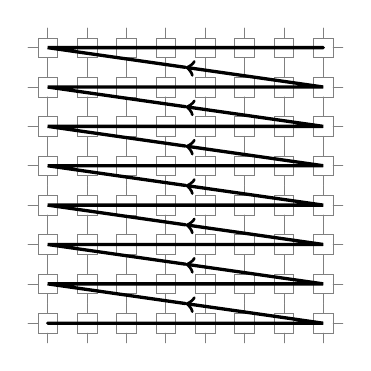
\begin{tikzpicture}[very thick, line cap=round, scale=0.5]
	
	\pgfmathtruncatemacro{\width}{8}
\pgfmathtruncatemacro{\height}{8}

\pgfmathtruncatemacro{\heightt}{\height-1}

% The topology
\begin{scope}[help lines]
	\foreach \x in {1,...,\width}{
		\foreach \y in {1,...,\height}{
			% Nodes
			\draw (\x-0.25, \y-0.25) rectangle ++(0.5, 0.5);
			
			% X axis links
			\draw (\x+0.25, \y) -- ++(0.25, 0);
			\draw (\x-0.25, \y) -- ++(-0.25, 0);
			% Y axis links
			\draw (\x, \y+0.25) -- ++(0, 0.25);
			\draw (\x, \y-0.25) -- ++(0, -0.25);
		}
	}
\end{scope}

	
	% Linear scan
	\foreach \y in {2,...,\heightt}{
		\draw [->]
		      (0.5*\width + 0.5, \y-0.5) --
		    ++(-0.5*\width+0.5, 0.5) --
		    ++(\width-1, 0) --
		    ++(-0.5*\width+0.5, 0.5)
		    ;
	}
	\draw [->]
	      (1, 1) --
	    ++(\width-1, 0) --
	    ++(-0.5*\width+0.5, 0.5)
	    ;
	\draw (0.5*\width + 0.5, \height - 0.5) --
	    ++(-0.5*\width+0.5, 0.5) --
	    ++(\width-1, 0)
	    ;
\end{tikzpicture}

